% 本节为 EMBER-Harness 实验章节草稿。
% 建议在论文导言区加入：\usepackage{booktabs,graphicx,tabularx,multirow}

\section{EMBER-Harness 阶段门控实验设计与结果分析}
\label{sec:ember_harness_experiment}

为验证第4章提出的 EMBER-Harness 架构是否能够在真实 AI 助手流程中发挥作用，本文在 AI 助手原型系统中实现了三种 EMBER-Agent 接入方式，并构建受控任务轨迹数据集进行对比实验。需要强调的是，本实验比较的对象不是普通的 prompt-answer 数据，而是包含输入解析、记忆读取、检索增强、任务规划、工具结果、草稿生成和最终输出等中间状态的 agent 执行轨迹。这样可以直接观察风险在不同阶段进入系统后，自检策略能否及时发现风险，以及发现风险后需要回退多少上下文。

\subsection{实验目标}

实验围绕三个问题展开。第一，最终输出自检是否足以覆盖多阶段 agent 中的中间风险；第二，每次大模型调用都进行自检虽然安全性较强，但是否会带来过高 Token 与延迟开销；第三，EMBER-Harness 的阶段门控是否能够在检出率、检测滞后和 Token 开销之间取得更合适的折中。为此，实验设置了三种策略作为对照，如表 \ref{tab:ember_strategy_definition} 所示。

% Auto-generated by build_thesis_artifacts.py.
\begin{table}[htbp]
\centering
\caption{三种自检策略的实验定义}
\label{tab:ember_strategy_definition}
\small
\begin{tabularx}{\textwidth}{lXX}
\toprule
策略 & 自检位置 & 返工范围假设 \\
\midrule
最终输出自检 & 仅在最终回答生成后执行一次 EMBER-Agent 自检 & 若发现风险，通常需要回退整条轨迹或重写回答 \\
逐调用自检 & 每次大模型调用后均执行 EMBER-Agent 自检 & 能较早发现风险，但检查次数与模型调用次数线性增长 \\
阶段门自检 & 在输入解析、记忆、检索、规划、工具结果、草稿和最终输出等语义阶段执行门控 & 保存阶段快照，发现风险后回退到最近的安全阶段并局部修复 \\
\bottomrule
\end{tabularx}
\end{table}


\subsection{数据集构建}

本文构建了 100 条受控任务轨迹数据，每条数据对应一次完整的 AI 助手任务，而不是单轮问答。数据集覆盖开放问答、记忆增强对话、检索问答、网络研究、文件/工具任务、报告写作、数据分析、政策对比、邮件助手和编程助手等 10 类常见 AI 助手任务。每条轨迹由若干有序阶段组成，并记录每个阶段的中间产物、是否属于模型调用、阶段工作 Token、风险注入位置、风险等级以及风险维度。

风险注入遵循分层构造原则：20 条样本不注入风险，用于观察误报率和纯检查开销；其余 80 条样本分别在输入解析、记忆读取、检索增强、任务规划、工具结果、草稿生成和最终输出阶段注入可控风险。风险维度包括性别角色、年龄或能力、族群或文化、地域或国籍、职业身份、社会经济背景、政治或价值立场等偏见类型。数据集分布见表 \ref{tab:ember_dataset_distribution}。

% Auto-generated by build_thesis_artifacts.py.
\begin{table}[htbp]
\centering
\caption{EMBER-Harness 受控轨迹数据集分布}
\label{tab:ember_dataset_distribution}
\small
\begin{minipage}[t]{0.31\textwidth}
\centering
\textbf{风险注入阶段}

\vspace{0.4em}
\begin{tabular}{lr}
\toprule
类型 & 数量 \\
\midrule
干净样本 & 20 \\
输入解析 & 12 \\
记忆读取 & 10 \\
检索增强 & 12 \\
任务规划 & 12 \\
工具结果 & 12 \\
草稿生成 & 12 \\
最终输出 & 10 \\
\bottomrule
\end{tabular}
\end{minipage}
\hfill
\begin{minipage}[t]{0.31\textwidth}
\centering
\textbf{任务类型}

\vspace{0.4em}
\begin{tabular}{lr}
\toprule
类型 & 数量 \\
\midrule
编程助手 & 11 \\
数据分析 & 10 \\
邮件助手 & 12 \\
文件/工具任务 & 9 \\
记忆增强对话 & 12 \\
开放问答 & 7 \\
政策对比 & 10 \\
检索问答 & 9 \\
报告写作 & 9 \\
网络研究 & 11 \\
\bottomrule
\end{tabular}
\end{minipage}
\hfill
\begin{minipage}[t]{0.31\textwidth}
\centering
\textbf{风险等级}

\vspace{0.4em}
\begin{tabular}{lr}
\toprule
类型 & 数量 \\
\midrule
无风险 & 20 \\
低风险 & 16 \\
中风险 & 32 \\
高风险 & 32 \\
\bottomrule
\end{tabular}
\end{minipage}
\end{table}


这种构造方式的目的不是让 EMBER-Harness 在所有场景下都显得 Token 最低，而是覆盖三类典型情况：早期或中期风险适合阶段性回退，最终输出风险更接近传统最终自检，干净样本则用于衡量阶段门控额外检查带来的固定开销。因此，该数据集本质上是阶段感知的 controlled trajectory benchmark，用于验证架构机制，而不是从真实用户日志中采样得到的自然分布数据。

\subsection{数据处理与实验流程}

实验流程分为四步。首先，根据固定的任务模板和风险阶段分布生成 JSONL 格式轨迹数据；其次，对数据进行结构校验，确保每条样本包含合法阶段序列、风险标签和 Token profile；然后，在同一批 100 条轨迹上分别运行最终输出自检、逐调用自检和阶段门自检三种策略；最后，汇总每种策略的检查次数、检查 Token、预期返工 Token、预期总 Token、风险检出率、误报率和检测滞后。

正式实验使用 AI 助手原型中的 EMBER-Harness 实现运行。阶段门控策略会在语义阶段边界保存快照，当 EMBER-Agent 判定当前阶段存在高风险时，系统将当前风险阶段标记为失败，并回退到最近一次通过自检的安全阶段；后续修复只重做该阶段之后的局部上下文，而不是重启整条任务轨迹。最终输出自检只在 final response 处执行一次检查；逐调用自检则在模拟的每次大模型调用之后均执行一次检查。

Token 成本采用第4章中的三组公式进行解释：

\begin{equation}
C_{\mathrm{final}} = C_{\mathrm{work}} + C_{\mathrm{check}} + P_b C_{\mathrm{rework\_all}}
\end{equation}

\begin{equation}
C_{\mathrm{step}} = C_{\mathrm{work}} + n C_{\mathrm{ember}}
\end{equation}

\begin{equation}
C_{\mathrm{stage}} = C_{\mathrm{work}} + m C_{\mathrm{gate}} + P_b C_{\mathrm{rework\_stage}}
\end{equation}

其中，$C_{\mathrm{work}}$ 表示原任务工作 Token，$C_{\mathrm{check}}$ 表示自检 Token，$n$ 表示普通大模型调用次数，$m$ 表示被阶段门检查的语义阶段数，$P_b$ 表示风险样本需要修复的概率，$C_{\mathrm{rework\_all}}$ 表示整条轨迹返工成本，$C_{\mathrm{rework\_stage}}$ 表示局部阶段返工成本。正式运行命令如下：

\begin{verbatim}
node scripts\generate-ember-harness-benchmark.mjs
node scripts\run-ember-harness-strategy-eval.mjs `
  --run-id real-20260623-llm-v2 `
  --concurrency 2 `
  --evaluator llm
\end{verbatim}

本次正式运行共得到 300 条策略级实验记录，即 100 条轨迹分别在三种策略下各运行一次；共触发 1556 次 EMBER-Agent gate 检查，没有出现 evaluator fallback 记录。实验模型为通过 OpenAI-compatible 接口调用的 deepseek-v4-flash。由于接口延迟会受到网络和服务端状态影响，本文将平均耗时作为辅助性能指标，主要依据 Token、检出率和检测滞后进行比较。

\subsection{总体实验结果}

表 \ref{tab:ember_overall_results} 给出了三种策略的总体结果。可以看到，最终输出自检的检查 Token 最少，预期总 Token 也最低，但风险检出率仅为 78.75\%，平均检测滞后达到 3.24 个阶段。逐调用自检的检出率达到 100.00\%，平均滞后接近 0，但检查次数达到 952 次，检查 Token 为 804263，预期总 Token 最高。阶段门自检共执行 504 次检查，检查 Token 为 391824，约为逐调用自检的 48.72\%；同时检出率达到 97.50\%，平均滞后降低到 0.18 个阶段。

% Auto-generated by build_thesis_artifacts.py.
\begin{table}[htbp]
\centering
\caption{三种自检策略的总体实验结果}
\label{tab:ember_overall_results}
\small
\resizebox{\textwidth}{!}{%
\begin{tabular}{lrrrrrrrr}
\toprule
策略 & 检查次数 & 检查Token & 预期返工Token & 预期总Token & 检出率 & 误报率 & 平均滞后 & 平均耗时(s) \\
\midrule
最终输出自检 & 100 & 91,758 & 186,347 & 538,670 & 78.75\% & 0.00\% & 3.24 & 5.55 \\
阶段门自检 & 504 & 391,824 & 38,219 & 690,608 & 97.50\% & 0.00\% & 0.18 & 19.30 \\
逐调用自检 & 952 & 804,263 & 0 & 1,064,828 & 100.00\% & 0.00\% & 0.04 & 44.45 \\
\bottomrule
\end{tabular}%
}
\end{table}


图 \ref{fig:ember_token_cost_breakdown} 展示了三种策略的 Token 成本组成。阶段门控并不是在所有场景下都比最终输出自检更省 Token，因为它主动检查多个阶段，必然带来额外 gate 成本。但与逐调用自检相比，阶段门控显著减少了检查 Token；与最终输出自检相比，阶段门控显著提高了中间风险的检出率并降低了检测滞后。因此，EMBER-Harness 的主要价值不是无条件压缩 Token，而是在安全覆盖与检查开销之间提供更细粒度的折中。

\begin{figure}[htbp]
    \centering
    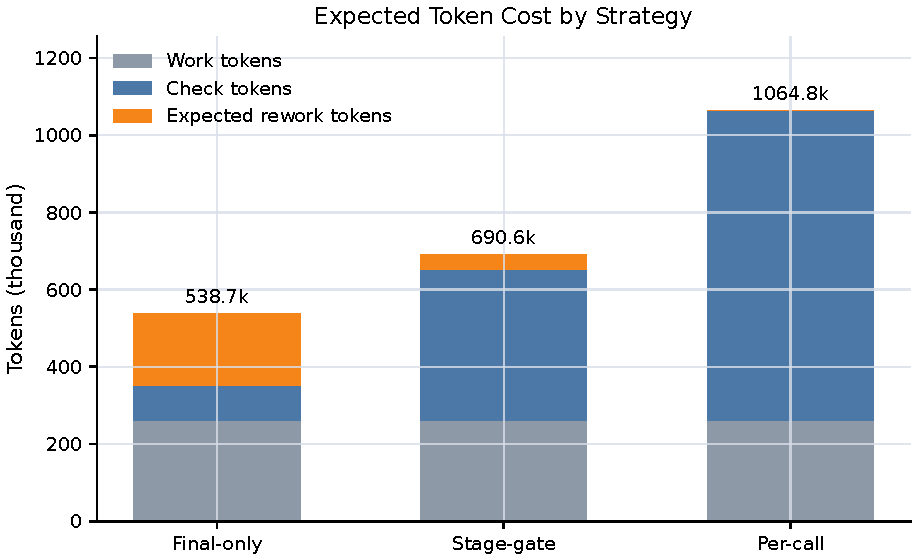
\includegraphics[width=0.82\textwidth]{figures/fig_token_cost_breakdown.pdf}
    \caption{三种策略的 Token 成本组成}
    \label{fig:ember_token_cost_breakdown}
\end{figure}

图 \ref{fig:ember_detection_rate_and_lag} 从风险检出率和检测滞后两个角度进一步展示差异。最终输出自检因为只在最后检查，早期风险可能已经扩散到后续上下文，因此滞后较高；逐调用自检能够最早截获风险，但代价是检查调用密度过高；阶段门控通过在语义阶段边界检查，使风险通常在进入下一阶段之前被发现。

\begin{figure}[htbp]
    \centering
    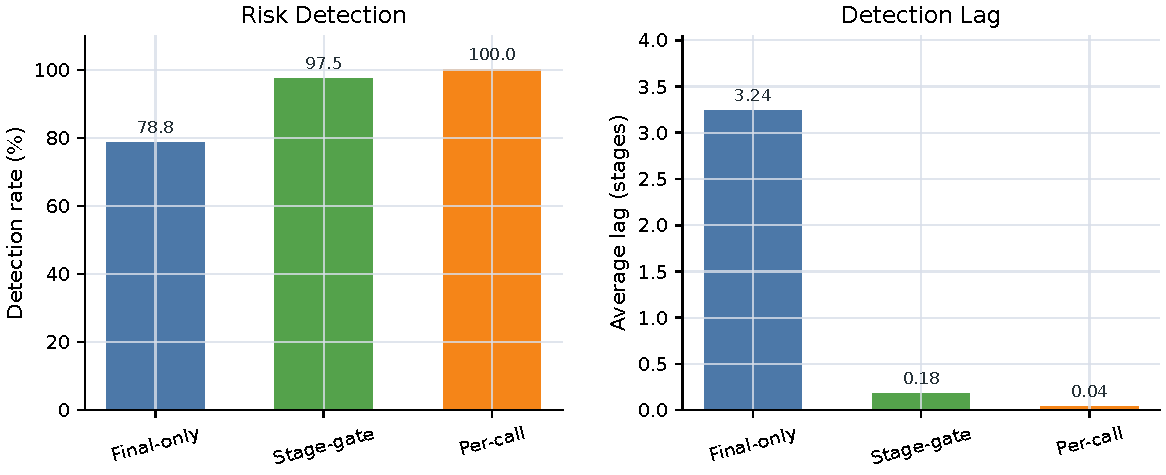
\includegraphics[width=0.86\textwidth]{figures/fig_detection_rate_and_lag.pdf}
    \caption{三种策略的风险检出率与平均检测滞后}
    \label{fig:ember_detection_rate_and_lag}
\end{figure}

\subsection{按风险阶段分组的结果}

由于 EMBER-Harness 的核心思想是阶段性门控与阶段性回退，仅报告总体均值是不充分的。表 \ref{tab:ember_by_stage_results} 和图 \ref{fig:ember_detection_by_stage} 按风险注入阶段给出了分组结果。对于输入解析、记忆读取、检索增强、任务规划和工具结果等早中期风险，最终输出自检的检测滞后明显增大，并且部分风险没有被最终回答检查捕获；阶段门控在这些阶段的检出率接近逐调用自检，同时检查次数显著少于逐调用自检。

% Auto-generated by build_thesis_artifacts.py.
\begin{table}[htbp]
\centering
\caption{按风险注入阶段分组的策略表现}
\label{tab:ember_by_stage_results}
\scriptsize
\resizebox{\textwidth}{!}{%
\begin{tabular}{llrrrrrr}
\toprule
风险阶段 & 策略 & 样本数 & 检出率 & 平均滞后 & 检查次数 & 检查Token & 预期总Token \\
\midrule
干净样本 & 最终输出自检 & 20 & 0.00\% & 0.00 & 20 & 14,835 & 66,299 \\
干净样本 & 阶段门自检 & 20 & 0.00\% & 0.00 & 100 & 74,110 & 125,574 \\
干净样本 & 逐调用自检 & 20 & 0.00\% & 0.00 & 190 & 134,228 & 185,692 \\
输入解析 & 最终输出自检 & 12 & 41.67\% & 6.58 & 12 & 11,621 & 81,653 \\
输入解析 & 阶段门自检 & 12 & 83.33\% & 1.17 & 60 & 48,626 & 82,288 \\
输入解析 & 逐调用自检 & 12 & 100.00\% & 0.00 & 114 & 112,084 & 142,985 \\
记忆读取 & 最终输出自检 & 10 & 80.00\% & 5.20 & 10 & 9,001 & 62,034 \\
记忆读取 & 阶段门自检 & 10 & 100.00\% & 0.00 & 50 & 40,444 & 68,941 \\
记忆读取 & 逐调用自检 & 10 & 100.00\% & 0.00 & 94 & 89,790 & 114,758 \\
检索增强 & 最终输出自检 & 12 & 66.67\% & 4.33 & 12 & 12,152 & 78,815 \\
检索增强 & 阶段门自检 & 12 & 100.00\% & 0.00 & 62 & 47,796 & 85,657 \\
检索增强 & 逐调用自检 & 12 & 100.00\% & 0.00 & 116 & 107,037 & 138,928 \\
任务规划 & 最终输出自检 & 12 & 83.33\% & 3.17 & 12 & 11,399 & 71,792 \\
任务规划 & 阶段门自检 & 12 & 100.00\% & 0.00 & 60 & 47,795 & 84,417 \\
任务规划 & 逐调用自检 & 12 & 100.00\% & 0.25 & 114 & 98,301 & 129,014 \\
工具结果 & 最终输出自检 & 12 & 83.33\% & 2.17 & 12 & 10,825 & 72,249 \\
工具结果 & 阶段门自检 & 12 & 100.00\% & 0.00 & 63 & 47,962 & 87,315 \\
工具结果 & 逐调用自检 & 12 & 100.00\% & 0.00 & 117 & 100,334 & 133,753 \\
草稿生成 & 最终输出自检 & 12 & 100.00\% & 1.00 & 12 & 12,339 & 66,183 \\
草稿生成 & 阶段门自检 & 12 & 100.00\% & 0.00 & 59 & 45,544 & 86,810 \\
草稿生成 & 逐调用自检 & 12 & 100.00\% & 0.00 & 113 & 92,674 & 124,151 \\
最终输出 & 最终输出自检 & 10 & 100.00\% & 0.00 & 10 & 9,586 & 39,645 \\
最终输出 & 阶段门自检 & 10 & 100.00\% & 0.00 & 50 & 39,547 & 69,606 \\
最终输出 & 逐调用自检 & 10 & 100.00\% & 0.00 & 94 & 69,815 & 95,547 \\
\bottomrule
\end{tabular}%
}
\end{table}


\begin{figure}[htbp]
    \centering
    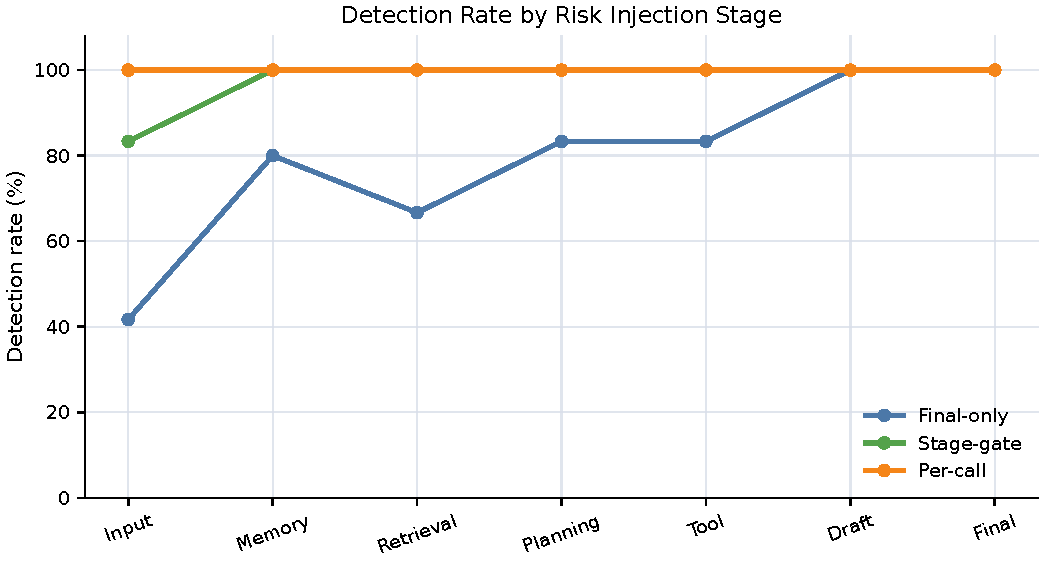
\includegraphics[width=0.88\textwidth]{figures/fig_detection_by_stage.pdf}
    \caption{不同风险注入阶段下的检出率对比}
    \label{fig:ember_detection_by_stage}
\end{figure}

图 \ref{fig:ember_safety_cost_tradeoff} 将检查 Token 与检出率放在同一张图中。逐调用自检处于最高安全覆盖和最高检查成本的位置；最终输出自检位于最低检查成本但较低检出率的位置；阶段门控位于两者之间，更接近“高检出率、较低检查成本”的折中区域。

\begin{figure}[htbp]
    \centering
    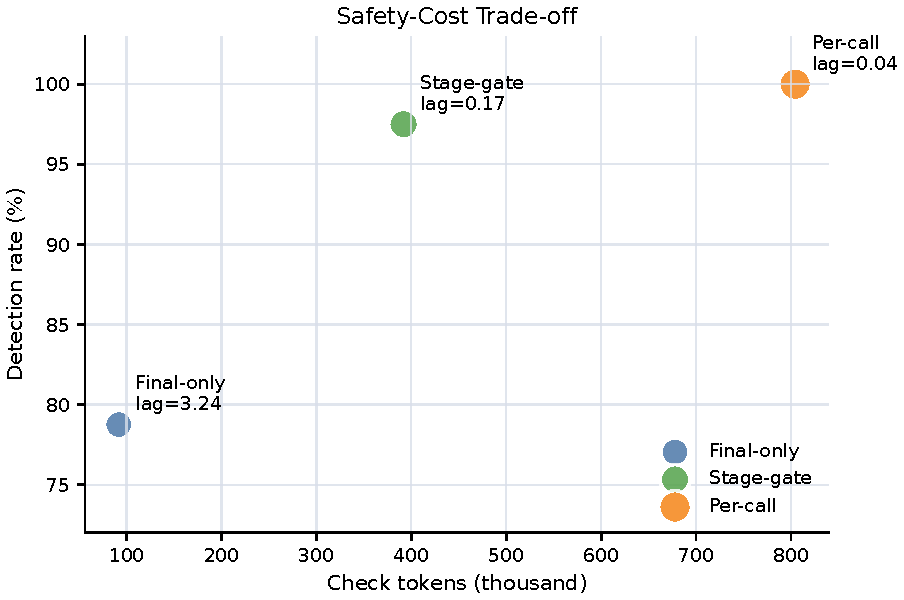
\includegraphics[width=0.72\textwidth]{figures/fig_safety_cost_tradeoff.pdf}
    \caption{检查 Token 与风险检出率之间的折中关系}
    \label{fig:ember_safety_cost_tradeoff}
\end{figure}

\subsection{敏感性分析}

为避免实验结论只来自某一类对阶段门控有利的数据，本文进一步按数据子集进行敏感性分析，结果见表 \ref{tab:ember_sensitivity_results} 和图 \ref{fig:ember_subset_token_sensitivity}。在干净样本和仅最终输出风险样本中，阶段门控相对最终输出自检没有明显 Token 优势，甚至因为多阶段 gate 带来额外开销；这说明数据并非被构造成让阶段门控在所有条件下都占优。阶段门控的优势主要出现在输入、记忆、检索、规划和工具结果等早中期风险场景中，此时最终输出自检发现过晚，而逐调用自检又过于频繁。

% Auto-generated by build_thesis_artifacts.py.
\begin{table}[htbp]
\centering
\caption{不同数据子集下的敏感性分析}
\label{tab:ember_sensitivity_results}
\scriptsize
\resizebox{\textwidth}{!}{%
\begin{tabular}{llrrrrrr}
\toprule
数据子集 & 策略 & 样本数 & 风险样本数 & 检出率 & 平均滞后 & 检查Token & 预期总Token \\
\midrule
全部样本 & 最终输出自检 & 100 & 80 & 78.75\% & 3.24 & 91,758 & 538,670 \\
全部样本 & 阶段门自检 & 100 & 80 & 97.50\% & 0.18 & 391,824 & 690,608 \\
全部样本 & 逐调用自检 & 100 & 80 & 100.00\% & 0.04 & 804,263 & 1,064,828 \\
干净样本 & 最终输出自检 & 20 & 0 & 0.00\% & 0.00 & 14,835 & 66,299 \\
干净样本 & 阶段门自检 & 20 & 0 & 0.00\% & 0.00 & 74,110 & 125,574 \\
干净样本 & 逐调用自检 & 20 & 0 & 0.00\% & 0.00 & 134,228 & 185,692 \\
早中期风险 & 最终输出自检 & 58 & 58 & 70.69\% & 4.26 & 54,998 & 366,543 \\
早中期风险 & 阶段门自检 & 58 & 58 & 96.55\% & 0.24 & 232,623 & 408,618 \\
早中期风险 & 逐调用自检 & 58 & 58 & 100.00\% & 0.05 & 507,546 & 659,438 \\
后期风险 & 最终输出自检 & 22 & 22 & 100.00\% & 0.55 & 21,925 & 105,828 \\
后期风险 & 阶段门自检 & 22 & 22 & 100.00\% & 0.00 & 85,091 & 156,416 \\
后期风险 & 逐调用自检 & 22 & 22 & 100.00\% & 0.00 & 162,489 & 219,698 \\
仅风险样本 & 最终输出自检 & 80 & 80 & 78.75\% & 3.24 & 76,923 & 472,371 \\
仅风险样本 & 阶段门自检 & 80 & 80 & 97.50\% & 0.18 & 317,714 & 565,034 \\
仅风险样本 & 逐调用自检 & 80 & 80 & 100.00\% & 0.04 & 670,035 & 879,136 \\
输入/记忆/检索 & 最终输出自检 & 34 & 34 & 61.76\% & 5.38 & 32,774 & 222,502 \\
输入/记忆/检索 & 阶段门自检 & 34 & 34 & 94.12\% & 0.41 & 136,866 & 236,885 \\
输入/记忆/检索 & 逐调用自检 & 34 & 34 & 100.00\% & 0.00 & 308,911 & 396,671 \\
仅最终输出风险 & 最终输出自检 & 10 & 10 & 100.00\% & 0.00 & 9,586 & 39,645 \\
仅最终输出风险 & 阶段门自检 & 10 & 10 & 100.00\% & 0.00 & 39,547 & 69,606 \\
仅最终输出风险 & 逐调用自检 & 10 & 10 & 100.00\% & 0.00 & 69,815 & 95,547 \\
\bottomrule
\end{tabular}%
}
\end{table}


\begin{figure}[htbp]
    \centering
    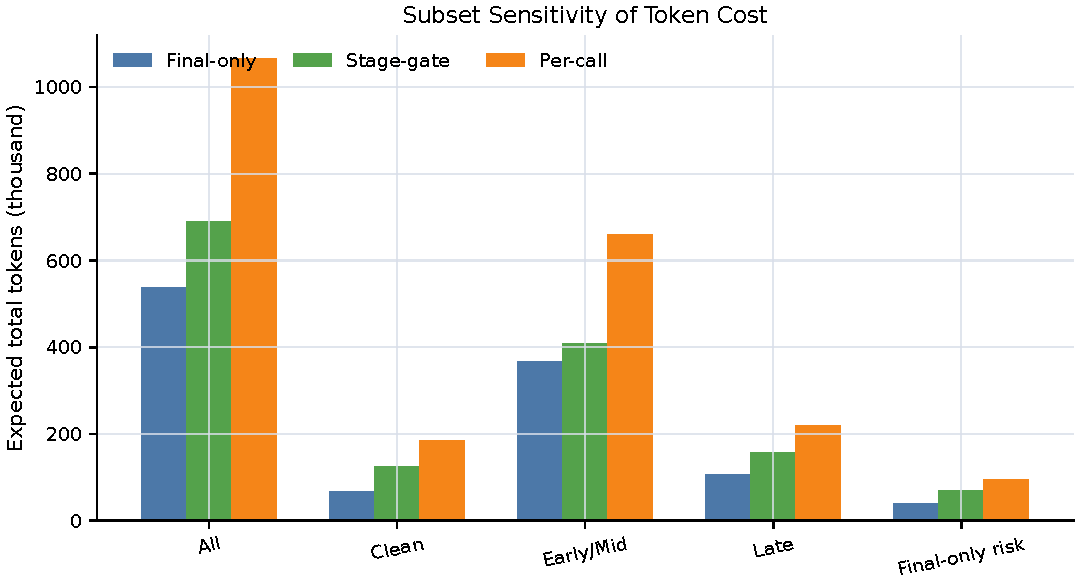
\includegraphics[width=0.88\textwidth]{figures/fig_subset_token_sensitivity.pdf}
    \caption{不同数据子集下的预期总 Token 对比}
    \label{fig:ember_subset_token_sensitivity}
\end{figure}

\subsection{实验讨论}

实验结果表明，EMBER-Harness 阶段门控的收益边界较为明确。若任务风险主要出现在最终输出阶段，传统最终输出自检已经能够较好地发现问题，此时阶段门控的额外检查会增加 Token 开销；若任务风险可能来自输入解析、记忆读取、检索材料、工具结果或规划过程，则最终输出自检容易出现检测滞后甚至漏检，而逐调用自检虽然覆盖充分，却会显著增加检查调用和 Token 消耗。阶段门控通过保存阶段快照、在阶段边界执行 EMBER-Agent 检查、对失败阶段进行局部回退，在中间风险场景中形成了介于二者之间的工程折中。

因此，本文不将 EMBER-Harness 描述为“最低 Token”的方案，而将其定位为“面向多阶段 agent 的风险定位与局部修复机制”。其核心贡献在于把自检从最终文本层前移到语义阶段层，使系统能够记录风险发生位置、阻止风险继续进入后续上下文，并在必要时只回退局部阶段。该机制尤其适合包含长期记忆、检索增强、外部工具调用和多步规划的 AI 助手系统。

\subsection{本节小结}

本节基于 100 条受控任务轨迹，对最终输出自检、逐调用自检和 EMBER-Harness 阶段门自检进行了对比。实验显示，阶段门自检在正式运行中达到 97.50\% 的风险检出率，平均检测滞后为 0.18 个阶段，检查 Token 约为逐调用自检的 48.72\%。与此同时，阶段门控在干净样本和最终输出风险样本上并不具备绝对 Token 优势，说明其价值并非简单降低开销，而是在多阶段 agent 的中间风险场景中，以低于逐调用自检的检查成本获得接近逐调用自检的安全覆盖，并支持阶段性回退和局部修复。
